\documentclass[10pt,aspectratio=43]{beamer}

% ============================================================
% Theme and style — match the Reference_Slides aesthetic
% ============================================================
\usetheme{default}
\usecolortheme{default}
\setbeamertemplate{navigation symbols}{}
\setbeamertemplate{footline}[frame number]

% Fonts
\usepackage{lmodern}
\usepackage[T1]{fontenc}

% Math
\usepackage{amsmath,amssymb,amsfonts}

% Tables and graphics
\usepackage{booktabs}
\usepackage{array}
\usepackage{graphicx}
\usepackage{tikz}
\usetikzlibrary{shapes,arrows,positioning,calc,decorations.pathreplacing}

% Colored boxes to match reference style
\usepackage{tcolorbox}
\tcbuselibrary{skins}

% Yellow highlight box (definitions, important concepts)
\newtcolorbox{yellowbox}{
  colback=yellow!20,
  colframe=yellow!20,
  boxrule=0pt,
  arc=0pt,
  left=4pt, right=4pt, top=4pt, bottom=4pt
}

% Red highlight box (key results, warnings)
\newtcolorbox{redbox}{
  colback=red!15,
  colframe=red!15,
  boxrule=0pt,
  arc=0pt,
  left=4pt, right=4pt, top=4pt, bottom=4pt
}

% Green highlight box (examples, positive notes)
\newtcolorbox{greenbox}{
  colback=green!10,
  colframe=green!10,
  boxrule=0pt,
  arc=0pt,
  left=4pt, right=4pt, top=4pt, bottom=4pt
}

% Slide number formatting: N/total
\setbeamertemplate{footline}{%
  \hfill\insertframenumber/\inserttotalframenumber\hspace*{6pt}\vspace*{4pt}%
}

% Remove default Beamer bullets, use simple bullets
\setbeamertemplate{itemize items}[circle]

% Page reference command: small gray note at bottom-left
\newcommand{\pref}[1]{\vfill\hfill{\scriptsize\color{gray}[Norton, pp.~#1]}}

% ============================================================
\title{Chapter 1: Introduction}
\subtitle{Design of Machinery --- Norton, 6th Edition}
\author{}
\date{}

\begin{document}

% ============================================================
% TITLE AND OVERVIEW
% ============================================================

\begin{frame}
\frametitle{Chapter 1: Introduction to Design of Machinery}

\begin{itemize}
  \item Purpose and scope of the textbook
  \item Kinematics and kinetics
  \item Mechanisms and machines
  \item A brief history of kinematics
  \item Applications of kinematics
  \item The engineering design process
  \item Units and dimensional analysis
  \item A design case study
\end{itemize}

\vspace{6pt}
\textbf{Related Reading}

Norton, \textit{Design of Machinery}, 6th ed., Chapter~1, pp.~3--29.
\end{frame}

% ============================================================
% 1.0 PURPOSE
% ============================================================

\begin{frame}
\frametitle{Purpose of This Course}

We will explore \textbf{kinematics} and \textbf{dynamics of machinery} with respect to:

\begin{yellowbox}
\begin{itemize}
  \item \textbf{Synthesis of mechanisms} --- create mechanisms to accomplish desired motions or tasks.
  \item \textbf{Analysis of mechanisms} --- determine the rigid-body dynamic behavior of existing mechanisms.
\end{itemize}
\end{yellowbox}

\vspace{6pt}
These topics are fundamental to the broader subject of \textbf{machine design}.

\vspace{6pt}
Key premise: \emph{We cannot analyze anything until it has been synthesized into existence.} Therefore we study synthesis first, then analysis.
\pref{3}
\end{frame}

% ============================================================
% 1.1 KINEMATICS AND KINETICS
% ============================================================

\begin{frame}
\frametitle{Kinematics and Kinetics}

\begin{yellowbox}
\textbf{Kinematics:} The study of motion \emph{without} regard to forces.

\textbf{Kinetics:} The study of forces on systems in motion.
\end{yellowbox}

\vspace{6pt}
These two concepts are \emph{not} physically separable. We arbitrarily separate them for instructional convenience.

\vspace{6pt}
From Newton's second law:
\[
  \mathbf{F} = m\,\mathbf{a}
\]
\begin{itemize}
  \item One typically needs the \textbf{accelerations}~($\mathbf{a}$) in order to compute the dynamic \textbf{forces}~($\mathbf{F}$).
  \item It is logical to study kinematics first, then kinetics.
\end{itemize}
\pref{3--4}
\end{frame}

\begin{frame}
\frametitle{The Role of Kinematics in Design}

One principal aim of \textbf{kinematics} is to create (design) the desired motions of mechanical parts and then mathematically compute positions, velocities, and accelerations.

\vspace{6pt}
\begin{redbox}
Since for most earthbound mechanical systems mass is essentially constant with time, defining the \textbf{accelerations} as a function of time also defines the \textbf{dynamic forces} as a function of time. Forces $\to$ stresses $\to$ service life.
\end{redbox}

\vspace{6pt}
In machinery that moves, the largest forces are often those due to the \textbf{dynamics of the machine itself}. These dynamic forces are proportional to acceleration, bringing us back to kinematics as the foundation.

\vspace{6pt}
\begin{yellowbox}
A design that has poor kinematics will prove troublesome and perform badly.
\end{yellowbox}
\pref{3--4}
\end{frame}

% ============================================================
% 1.2 MECHANISMS AND MACHINES
% ============================================================

\begin{frame}
\frametitle{Mechanisms and Machines}

\begin{yellowbox}
\textbf{Mechanism:} A system of elements arranged to transmit motion \emph{in a predetermined fashion}. Transforms motion, develops low forces, transmits little power.
\end{yellowbox}

\vspace{4pt}
\begin{yellowbox}
\textbf{Machine:} A mechanism (or collection of mechanisms) designed to provide significant \textbf{forces} and transmit significant \textbf{power}. Add the words ``and energy'' after motion.
\end{yellowbox}

\vspace{6pt}
\textbf{Examples of mechanisms:} pencil sharpener, camera shutter, analog clock, folding chair, adjustable desk lamp, umbrella.

\vspace{4pt}
\textbf{Examples of machines:} food blender, bank vault door, automobile transmission, bulldozer, robot, amusement park ride.

\vspace{6pt}
The dividing line is \emph{not} clear-cut; they differ in degree rather than kind. If forces/energy are significant $\to$ machine; if not $\to$ mechanism.
\pref{4--5}
\end{frame}

\begin{frame}
\frametitle{Analysis Strategy for Mechanisms vs.\ Machines}

\begin{itemize}
  \item Mechanisms (lightly loaded, slow speeds) can sometimes be treated as \textbf{purely kinematic} devices --- analyze without regard to forces.
  \item Machines (and mechanisms at higher speeds) must first be treated as mechanisms:
  \begin{enumerate}
    \item Kinematic analysis of velocities and accelerations.
    \item Subsequently analyzed as \textbf{dynamic systems} --- static and dynamic forces using the principles of kinetics.
  \end{enumerate}
\end{itemize}

\vspace{6pt}
\begin{yellowbox}
\textbf{Part~I} of the text: \textbf{Kinematics of Mechanisms}

\textbf{Part~II} of the text: \textbf{Dynamics of Machinery}

The synthesis techniques in Part~I apply to \emph{both} mechanisms and machines.
\end{yellowbox}
\pref{4--5}
\end{frame}

% ============================================================
% 1.3 A BRIEF HISTORY OF KINEMATICS
% ============================================================

\begin{frame}
\frametitle{A Brief History of Kinematics}

Machines and mechanisms have been devised since the dawn of history.

\vspace{4pt}
\textbf{Ancient period:}
\begin{itemize}
  \item Egyptians: lever, inclined plane (wedge), log roller. Wheel and axle \emph{not} known to Old Kingdom Egyptians.
  \item First wheel \& axle: Mesopotamia, ca.\ 3000--4000 B.C.
  \item Early machine design focused on military applications (catapults, wall scaling, etc.).
\end{itemize}

\vspace{4pt}
\textbf{Industrial revolution:}
\begin{itemize}
  \item \textbf{James Watt} (1736--1819): first kinematician; synthesized a straight-line linkage to guide steam engine pistons.
  \item \textbf{Oliver Evans} (1755--1819): designed a straight-line linkage for a steam engine.
  \item \textbf{Euler} (1707--1783): analytical treatment of mechanisms; concept that planar motion $=$ translation $+$ rotation.
\end{itemize}
\pref{5--6}
\end{frame}

\begin{frame}
\frametitle{History of Kinematics (continued)}

\textbf{19th century formalization:}
\begin{itemize}
  \item L'Ecole Polytechnic, Paris: \textbf{Lagrange}, \textbf{Fourier}, \textbf{Gaspard Monge} (descriptive geometry).
  \item \textbf{Hachette} (1806): first mechanism text.
  \item \textbf{Andr\'e Marie Ampere} (1775--1836): coined the term \textbf{cin\'ematique} (kinematics) --- from Greek $\kappa\iota\nu\eta\mu\alpha$ (motion).
  \item \textbf{Robert Willis} (1841): \emph{Principles of Mechanism}; five ways to obtain relative motion between input and output links.
  \item \textbf{Franz Reuleaux} (1829--1905): \emph{Theoretische Kinematik} (1875). Defined six basic mechanical components: link, wheel, cam, screw, ratchet, belt. Father of modern kinematics.
\end{itemize}

\vspace{4pt}
\textbf{20th century (post-WWII):}
\begin{itemize}
  \item \textbf{A.\ E.\ R.\ de Jonge} (1940s): called attention to kinematics in the U.S.
  \item \textbf{Freudenstein, Denavit, Erdman, Hall, Hartenberg, Sandor, Soni}: American and European contributions to kinematic synthesis.
  \item Computers enabled solving previously intractable problems.
\end{itemize}
\pref{5--6}
\end{frame}

% ============================================================
% 1.4 APPLICATIONS OF KINEMATICS
% ============================================================

\begin{frame}
\frametitle{Applications of Kinematics}

The first task in any machine design problem: determine the \textbf{kinematic configuration} needed to provide the desired motions.

\vspace{4pt}
\begin{yellowbox}
Force and stress analyses typically \emph{cannot} be done until kinematic issues are resolved. This text addresses: \textbf{linkages}, \textbf{cams}, and \textbf{gears}.
\end{yellowbox}

\vspace{6pt}
Virtually any machine or device that moves contains kinematic elements:
\begin{itemize}
  \item \textbf{Bicycle:} chain drive (torque multiplication), cable-operated linkages (braking).
  \item \textbf{Automobile:} steering system, wheel suspensions, piston engine (linkages), valves (cams), transmission (gears), windshield wipers (linkage-driven).
  \item \textbf{Construction equipment:} tractors, cranes, backhoes all use linkages extensively, often driven by hydraulic cylinders.
  \item \textbf{Consumer goods:} exercise equipment, office chairs, folding mechanisms.
\end{itemize}
\pref{6--7}
\end{frame}

% ============================================================
% 1.5 A DESIGN PROCESS
% ============================================================

\begin{frame}
\frametitle{The Engineering Design Process}

\begin{yellowbox}
\textbf{Engineering design:} The creation of a device, system, or process using engineering principles. It involves both \textbf{synthesis} (putting together) and \textbf{analysis} (taking apart).
\end{yellowbox}

\vspace{4pt}
Real design problems are \textbf{unstructured} --- they lead to ``blank paper syndrome.'' The design process provides structure.

\vspace{6pt}
\textbf{Key property: Iteration}
\begin{itemize}
  \item The design process is \emph{not} linear (steps 1 through 10).
  \item It is inherently \textbf{circular}. To \textbf{iterate} means \emph{to repeat, to return to a previous state.}
  \item Progress is made haltingly: two steps forward, one step back.
\end{itemize}
\pref{7--8}
\end{frame}

\begin{frame}
\frametitle{The 10-Step Design Process}

\begin{center}
\begin{tabular}{cl}
\toprule
\textbf{Step} & \textbf{Activity} \\
\midrule
1 & Identification of Need \\
2 & Background Research \\
3 & Goal Statement \\
4 & Performance Specifications \\
5 & Ideation and Invention \\
6 & Analysis \\
7 & Selection \\
8 & Detailed Design \\
9 & Prototyping and Testing \\
10 & Production \\
\bottomrule
\end{tabular}
\end{center}

\vspace{6pt}
\begin{redbox}
Remember: this process is \textbf{iterative}. At any step you may need to return to an earlier step. The actual execution is circular, not sequential.
\end{redbox}
\pref{8; Table 1-1}
\end{frame}

\begin{frame}
\frametitle{Step 1: Identification of Need}

This step is often initiated by someone saying: ``What we need is \ldots''

\vspace{6pt}
\begin{itemize}
  \item Typically a brief, vague statement.
  \item Falls far short of a structured problem statement.
  \item Example: ``We need a better lawn mower.''
\end{itemize}

\vspace{6pt}
\begin{redbox}
\textbf{Warning:} This statement is almost never a well-defined problem. The real engineering challenge is \textbf{structuring the unstructured problem}. Many excellent solutions have been rejected because they solved \emph{the wrong problem}.
\end{redbox}

\vspace{6pt}
Before any attempt to \emph{solve} the problem, you must first carefully \textbf{define} the problem using an engineering approach.
\pref{8}
\end{frame}

\begin{frame}
\frametitle{Step 2: Background Research}

\begin{redbox}
This is the \textbf{most important} phase in the design process, and unfortunately the most \textbf{neglected}.
\end{redbox}

\vspace{6pt}
The goal: gather background information on the relevant physics, chemistry, or other aspects of the problem. Has this (or a similar) problem been solved before?

\vspace{6pt}
\textbf{Key resources:}
\begin{itemize}
  \item \textbf{Patent literature} (USPTO: \texttt{www.uspto.gov}) --- search by keyword, inventor, title. The ``disclosure'' section describes the invention in full detail.
  \item \textbf{Technical publications} --- ASME journals, IFToMM, \emph{Mechanism and Machine Theory}.
  \item \textbf{Benchmarking} --- purchase, disassemble, and analyze competitors' products.
  \item \textbf{Web resources} --- vast amount of machine design information.
\end{itemize}

\vspace{4pt}
\begin{yellowbox}
Do \emph{not} skip this step! Avoid ``reinventing the wheel.'' Invest sufficient time in research \emph{before} ideation.
\end{yellowbox}
\pref{9}
\end{frame}

\begin{frame}
\frametitle{Step 3: Goal Statement}

Once the background is understood, recast the problem as a coherent \textbf{goal statement}. Three characteristics:
\begin{enumerate}
  \item \textbf{Concise} and \textbf{general}
  \item \textbf{Uncolored} by terms that predict a solution
  \item Couched in terms of \textbf{functional visualization} --- meaning to visualize \emph{function}, not a particular embodiment
\end{enumerate}

\vspace{6pt}
\textbf{Example:}
\begin{itemize}
  \item \textbf{Bad:} ``Design a Better Lawn Mower.'' (Implies a specific type of device.)
  \item \textbf{Good:} ``Design a Means to Shorten Grass.'' (Opens up creative possibilities.)
\end{itemize}

\vspace{4pt}
\begin{yellowbox}
Use \textbf{functional visualization} to avoid unnecessarily limiting your creativity! The phrase ``lawn mower'' conjures images of whirring blades and a noisy engine. ``Shorten grass'' opens up 10+ alternative approaches.
\end{yellowbox}
\pref{10}
\end{frame}

\begin{frame}
\frametitle{Step 4: Performance Specifications}

Once the goal is clearly stated, formulate \textbf{performance specifications} (also called task specifications).

\begin{yellowbox}
\textbf{Performance specifications} define \emph{what the system must do}.

\textbf{Design specifications} define \emph{how it must do it}.

At this stage, specify \textbf{what}, not \textbf{how}. Leave the ``how'' for the ideation phase.
\end{yellowbox}

\vspace{6pt}
\textbf{Example:} ``Design a Means to Shorten Grass''
\begin{enumerate}
  \item Device to have self-contained power supply.
  \item Device to be corrosion resistant.
  \item Device to cost less than \$100.
  \item Device to emit $<80$~dB at 10\,m.
  \item Device to shorten 1/4~acre of grass per hour.
\end{enumerate}

\vspace{4pt}
These constrain the design \emph{without} overly restricting the engineer's freedom. (E.g., requiring a gasoline engine would be inappropriate.)
\pref{10; Table 1-2}
\end{frame}

\begin{frame}
\frametitle{Step 5: Ideation and Invention}

This is potentially the most \textbf{satisfying} step, but also the most \textbf{difficult}.

\vspace{4pt}
\begin{yellowbox}
\textbf{The Creative Process} (Table 1-3 in text):
\begin{enumerate}
  \item[5a.] \textbf{Idea Generation}
  \item[5b.] \textbf{Frustration}
  \item[5c.] \textbf{Incubation}
  \item[5d.] \textbf{Eureka!}
\end{enumerate}
\end{yellowbox}

\vspace{4pt}
\textbf{Idea Generation:} The most important technique is \textbf{deferred judgment} --- do not judge quality at this stage. Aim for \emph{quantity}.

\vspace{4pt}
\textbf{Useful techniques:}
\begin{itemize}
  \item \textbf{Brainstorming} (6--15 people, no criticism, one ``scribe'').
  \item \textbf{Analogies and inversion} --- convert between problem domains; turn the problem inside out.
  \item \textbf{Synonyms} --- define the action verb, then list synonyms.
\end{itemize}
\pref{10--11; Table 1-3}
\end{frame}

\begin{frame}
\frametitle{The Creative Process: Frustration Through Eureka}

\textbf{Problem statement:} \emph{Move this object from point A to point B.}

Action verb: ``move.'' Synonyms: push, pull, slip, slide, shove, throw, eject, jump, spill.

\vspace{6pt}
\textbf{Frustration:} At some point your ``mental well'' goes dry. This is normal.

\vspace{4pt}
\textbf{Incubation:} Leave the problem and do something else. Your subconscious continues to work on it.

\begin{redbox}
\textbf{Eureka!} At a quite unexpected time and place, an idea will pop into your consciousness. It will seem to be the obvious and ``right'' solution.

Most likely, later analysis will find flaws. \textbf{Iterate!} Back up and repeat.
\end{redbox}

\vspace{4pt}
Three requirements for creative insight (Wallen):
\begin{enumerate}
  \item Fascination with the problem.
  \item Saturation with the facts and background.
  \item A period of reorganization (incubation).
\end{enumerate}
\pref{11--12}
\end{frame}

\begin{frame}
\frametitle{Step 6: Analysis}

Once you have structured the problem (at least temporarily), apply more sophisticated \textbf{analysis techniques} to examine performance.

\vspace{6pt}
\begin{itemize}
  \item Some analysis methods will be discussed in detail in the following chapters (position, velocity, acceleration, force analysis).
  \item Further \textbf{iteration} will be required as problems are discovered.
  \item Repetition of earlier steps is necessary to ensure the success of the design.
\end{itemize}

\vspace{6pt}
A useful tool: the \textbf{Decision Matrix} (weighted scoring method).

\vspace{4pt}
\begin{yellowbox}
Rows $=$ design alternatives. Columns $=$ evaluation categories (cost, safety, performance, reliability, \ldots). Each column has a \textbf{weighting factor}. Scores are subjective (1--10 scale), then weighted and summed for each design.
\end{yellowbox}
\pref{12}
\end{frame}

\begin{frame}
\frametitle{The Decision Matrix}

\begin{center}
\small
\begin{tabular}{l|c|c|c|c|c}
\toprule
 & \textbf{Cost} & \textbf{Safety} & \textbf{Perform.} & \textbf{Reliab.} & \textbf{Rank} \\
\textit{Weight} & 0.35 & 0.30 & 0.15 & 0.20 & 1.0 \\
\midrule
Design 1 & 3 / 1.05 & 4 / 1.20 & 9 / 1.35 & 6 / 1.20 & \textbf{4.8} \\
Design 2 & 4 / 1.40 & 2 / 0.60 & 7 / 1.05 & 2 / 0.40 & 3.5 \\
Design 3 & 1 / 0.35 & 9 / 2.70 & 4 / 0.60 & 5 / 1.00 & 4.7 \\
Design 4 & 9 / 3.15 & 1 / 0.30 & 6 / 0.90 & 7 / 1.40 & \textbf{5.8} \\
Design 5 & 7 / 2.45 & 4 / 1.20 & 2 / 0.30 & 6 / 1.20 & 5.2 \\
\bottomrule
\end{tabular}
\end{center}

\vspace{6pt}
\begin{redbox}
\textbf{Caution:} The scores and weightings are \emph{subjective}. The real value of the decision matrix is that it forces you to think systematically about the relative merits of each design across multiple categories. Do not put too much faith in the decimal places!
\end{redbox}
\pref{12; Fig.~1-2}
\end{frame}

\begin{frame}
\frametitle{Step 7: Selection}

When the analysis indicates several potentially viable designs, select the best one for:
\begin{itemize}
  \item \textbf{Detailed design}
  \item \textbf{Prototyping}
  \item \textbf{Testing}
\end{itemize}

\vspace{6pt}
The selection process usually involves a comparative analysis of the available design solutions (e.g., the decision matrix).

\vspace{6pt}
The decision matrix helps identify the best solution by systematically considering \textbf{cost}, \textbf{ease of use}, \textbf{efficiency}, \textbf{performance}, \textbf{reliability}, and other factors with appropriate weighting.
\pref{13}
\end{frame}

\begin{frame}
\frametitle{Steps 8--10: Detailed Design, Prototyping, Production}

\textbf{Step 8 --- Detailed Design:}
\begin{itemize}
  \item Create complete assembly and detail drawings or \textbf{CAD} part files.
  \item Every dimension, material specification must be included.
  \item Flaws found here require further \textbf{iteration}.
\end{itemize}

\vspace{6pt}
\textbf{Step 9 --- Prototyping and Testing:}
\begin{itemize}
  \item Build a prototype physical model (mathematical models are useful but never as complete as a physical model).
  \item Test: measure displacements, velocities, accelerations, forces, temperatures, etc.
  \item \textbf{Simple cardboard models} of linkages (joined with thumbtacks for pivots) are very informative!
\end{itemize}

\vspace{6pt}
\textbf{Step 10 --- Production:}
\begin{itemize}
  \item Manufacture the final version.
  \item Danger of finding flaws after producing thousands of units should motivate care in earlier steps.
\end{itemize}
\pref{13--14}
\end{frame}

\begin{frame}
\frametitle{The Design Process is Iterative}

\begin{center}
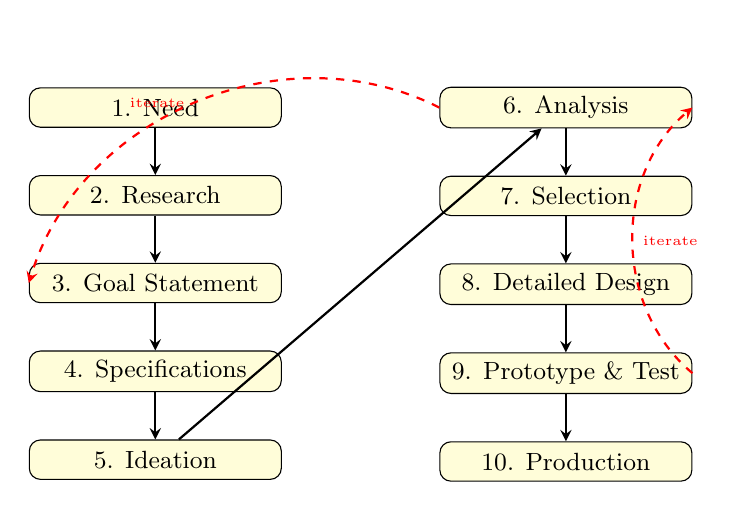
\begin{tikzpicture}[
  node distance=0.6cm,
  box/.style={draw, rounded corners, minimum width=3.2cm, minimum height=0.5cm, font=\small, fill=yellow!15},
  arrow/.style={->, thick, >=stealth}
]
\node[box] (n1) {1. Need};
\node[box, below=of n1] (n2) {2. Research};
\node[box, below=of n2] (n3) {3. Goal Statement};
\node[box, below=of n3] (n4) {4. Specifications};
\node[box, below=of n4] (n5) {5. Ideation};
\node[box, right=2cm of n1] (n6) {6. Analysis};
\node[box, below=of n6] (n7) {7. Selection};
\node[box, below=of n7] (n8) {8. Detailed Design};
\node[box, below=of n8] (n9) {9. Prototype \& Test};
\node[box, below=of n9] (n10) {10. Production};

\foreach \a/\b in {n1/n2, n2/n3, n3/n4, n4/n5, n5/n6, n6/n7, n7/n8, n8/n9, n9/n10}
  \draw[arrow] (\a) -- (\b);

% Iteration arrows (going back)
\draw[arrow, red, dashed, bend right=50] (n6.west) to node[left, font=\tiny, red]{iterate} (n3.west);
\draw[arrow, red, dashed, bend left=50] (n9.east) to node[right, font=\tiny, red]{iterate} (n6.east);
\end{tikzpicture}
\end{center}

\end{frame}

\begin{frame}
\frametitle{Engineering as a Discipline}

\begin{yellowbox}
\textbf{Engineering} is as much a \emph{method}, an \emph{approach}, a \emph{process}, a \emph{state of mind for problem solving}, as it is an activity.
\end{yellowbox}

\vspace{6pt}
The engineering approach requires:
\begin{itemize}
  \item \textbf{Thoroughness} and \textbf{attention to detail}
  \item \textbf{Open-minded, freewheeling creative thinking}
  \item These are not contradictory --- they are \textbf{symbiotic}
\end{itemize}

\vspace{6pt}
To do a creditable job in the design of anything:
\begin{itemize}
  \item You must \emph{completely} define the problem.
  \item You must \emph{thoroughly} research the background.
  \item You must \emph{exhaustively} pursue conceptual solutions.
  \item You must \emph{extensively} analyze for validity.
  \item You must \emph{detail} down to the last nut and bolt.
\end{itemize}
\pref{14}
\end{frame}

% ============================================================
% 1.6 OTHER APPROACHES TO DESIGN
% ============================================================

\begin{frame}
\frametitle{Other Approaches to Design}

\textbf{Dixon's information-based view:}
\begin{itemize}
  \item A design is a \emph{state of information} that evolves from abstract $\to$ detailed.
  \item Several states: \textbf{requirements} $\approx$ performance specs; \textbf{conceptual} $\approx$ ideation; \textbf{feature configuration / parametric} $\approx$ detailed design.
  \item Design $=$ ``the series of activities by which information about the designed object is changed from one state to another.''
\end{itemize}

\vspace{6pt}
\textbf{Suh's Axiomatic Design} --- two axioms:
\begin{yellowbox}
\begin{enumerate}
  \item \textbf{Maintain the independence} of the functional requirements.
  \item \textbf{Minimize the information content} (least complexity).
\end{enumerate}
\end{yellowbox}

\vspace{4pt}
The second axiom is sometimes stated as \textbf{KISS}: \emph{Keep It Simple, Stupid.}
\pref{15}
\end{frame}

% ============================================================
% 1.7 MULTIPLE SOLUTIONS
% ============================================================

\begin{frame}
\frametitle{Multiple Solutions}

\begin{redbox}
By the nature of the design process, there is \textbf{not} any one correct answer or solution to any design problem. Unlike textbook problems, there is no answer ``in the back of the book.''
\end{redbox}

\vspace{6pt}
\begin{itemize}
  \item There are as many potential solutions as there are designers willing to attempt them.
  \item Some will be better than others, but \textbf{many will work}.
  \item The only way to assess relative merit: thorough analysis and physical testing.
  \item Where feasible, create \textbf{mathematical models} and solve on the computer before building prototypes.
\end{itemize}

\vspace{6pt}
In mechanism design:
\begin{itemize}
  \item Usually possible to write the equations for rigid-body dynamics and solve in ``closed form'' (with or without a computer).
  \item Elastic deformations: \textbf{finite difference} or \textbf{finite element method} (FEM).
\end{itemize}
\pref{16}
\end{frame}

% ============================================================
% 1.8 HUMAN FACTORS ENGINEERING
% ============================================================

\begin{frame}
\frametitle{Human Factors Engineering}

With few exceptions, all machines are designed to be used by humans (even robots must be programmed by a human).

\begin{yellowbox}
\textbf{Human factors engineering} (also \textbf{ergonomics}) is defined as \emph{an applied science that coordinates the design of devices, systems, and physical working conditions with the capacities and requirements of the worker}.
\end{yellowbox}

\vspace{6pt}
Design philosophy: ``Fit the machine to the man,'' \emph{not} ``fit the man to the machine.''

\vspace{6pt}
Data needed for machine design:
\begin{itemize}
  \item Dimensions of the human body (by age, gender).
  \item Ability to withstand accelerations in various directions.
  \item Typical strengths and force-generating ability.
  \item Noise tolerance limits.
  \item Reach envelopes and visual field constraints.
\end{itemize}
\pref{16}
\end{frame}

% ============================================================
% 1.9 THE ENGINEERING REPORT
% ============================================================

\begin{frame}
\frametitle{The Engineering Report}

\begin{redbox}
Communication of ideas and results is a \textbf{very important} aspect of engineering. Engineers spend the largest percentage of their time communicating with others --- orally or in writing.
\end{redbox}

\vspace{6pt}
\begin{itemize}
  \item The usual form of presentation: a formal \textbf{engineering report}.
  \item \emph{You may be the cleverest person in the world, but no one will know that if you cannot communicate your ideas clearly and concisely.}
  \item If you cannot explain what you have done, you probably don't understand it yourself.
\end{itemize}

\vspace{6pt}
Design project assignments in later chapters are intended to give you experience in writing formal engineering reports.
\pref{17}
\end{frame}

% ============================================================
% 1.10 UNITS
% ============================================================

\begin{frame}
\frametitle{Systems of Units}

Three common systems, all derived from Newton's second law:
\[
  F = \frac{m \, l}{t^2}
\]
where $F$ = force, $m$ = mass, $l$ = length, $t$ = time.

\vspace{6pt}
For any three of these variables, choose base units; the fourth is derived.

\begin{center}
\small
\begin{tabular}{l|ccc}
\toprule
 & \textbf{fps} & \textbf{ips} & \textbf{SI} \\
\midrule
Length & feet (ft) & inches (in) & meters (m) \\
Force & pounds (lb) & pounds (lb) & \textit{newtons (N)} \\
Time & seconds (sec) & seconds (sec) & seconds (sec) \\
Mass & \textit{slugs (sl)} & \textit{blobs (bl)} & kilograms (kg) \\
\midrule
Base units & $F, l, t$ & $F, l, t$ & $m, l, t$ \\
Derived unit & mass & mass & force \\
Type & gravitational & gravitational & absolute \\
\bottomrule
\end{tabular}
\end{center}
\pref{17}
\end{frame}

\begin{frame}
\frametitle{U.S.\ Foot-Pound-Second (fps) System}

\textbf{Base units:} feet (ft), pounds (lb), seconds (sec).

Mass is derived from Newton's law:
\[
  m = \frac{F \, t^2}{l} \quad \Longrightarrow \quad \text{lb-sec}^2/\text{ft} = \textbf{slugs (sl)}
\]

\vspace{6pt}
\textbf{U.S.\ Inch-Pound-Second (ips) System:}

\textbf{Base units:} inches (in), pounds (lb), seconds (sec).
\[
  m = \frac{F \, t^2}{l} \quad \Longrightarrow \quad \text{lb-sec}^2/\text{in} = \textbf{blobs (bl)}
\]

\begin{redbox}
\textbf{Critical:} 1 blob = 12 slugs. If you measure lengths in \textbf{inches} and then use $g = 32.2$ \textbf{feet}/sec$^2$ to compute mass, you will have an error of a \textbf{factor of twelve}. This is enough to crash the airplane you designed!
\end{redbox}
\pref{17--18}
\end{frame}

\begin{frame}
\frametitle{Weight vs.\ Mass}

Weight is defined as the force exerted on an object by gravity:
\[
  m = \frac{W}{g}
\]

\begin{yellowbox}
\textbf{Key values:}

fps: $g \approx 32.2$ ft/sec$^2$

ips: $g \approx 386$ in/sec$^2$

SI: $g \approx 9.81$ m/s$^2$
\end{yellowbox}

\vspace{4pt}
The most common student error: mixing fps and ips units when computing mass.

\vspace{6pt}
\textbf{Pounds mass (lb$_m$):} Used in fluid dynamics and thermodynamics. The value of mass in lb$_m$ is \emph{numerically} equal to its weight in lb$_f$. But you \textbf{must} divide by $g_c$ when using Newton's equation:
\[
  F = \frac{m\,a}{g_c}
\]
where $g_c$ is the gravitational constant (32.2 or 386 depending on system).
\pref{18}
\end{frame}

\begin{frame}
\frametitle{The SI System}

\textbf{Base units:} mass (kg), length (m), time (sec).

Force is the \textbf{derived} unit:
\[
  \text{kg} \cdot \text{m/s}^2 = \textbf{newtons (N)}
\]

\begin{yellowbox}
\textbf{Advantage of SI:} Mass is a base unit whose value is independent of local gravity. This is an \textbf{absolute} system (vs.\ the U.S.\ \textbf{gravitational} systems).

In SI, there are distinct names for mass (kg) and force (N), which helps alleviate confusion.
\end{yellowbox}

\vspace{6pt}
\textbf{Converting between systems:}
\begin{itemize}
  \item Mass: kg $\to$ slugs (sl) or blobs (bl)
  \item Force: newtons (N) $\to$ pounds (lb)
  \item $g \approx 9.81$ m/s$^2$
\end{itemize}
\pref{18--19}
\end{frame}

\begin{frame}
\frametitle{Variables and Units (Table 1-4)}

\begin{center}
\small
\begin{tabular}{l|c|c|c|c}
\toprule
\textbf{Variable} & \textbf{Symbol} & \textbf{ips} & \textbf{fps} & \textbf{SI} \\
\midrule
Force & $F$ & \textbf{lb} & \textbf{lb} & \textbf{N} \\
Length & $l$ & \textbf{in} & \textbf{ft} & \textbf{m} \\
Time & $t$ & \textbf{sec} & \textbf{sec} & \textbf{sec} \\
Mass & $m$ & bl & sl & \textbf{kg} \\
Velocity & $v$ & in/sec & ft/sec & m/sec \\
Acceleration & $a$ & in/sec$^2$ & ft/sec$^2$ & m/sec$^2$ \\
Jerk & $j$ & in/sec$^3$ & ft/sec$^3$ & m/sec$^3$ \\
Angle & $\theta$ & deg / rad & deg / rad & deg / rad \\
Angular velocity & $\omega$ & rad/sec & rad/sec & rad/sec \\
Angular accel.\ & $\alpha$ & rad/sec$^2$ & rad/sec$^2$ & rad/sec$^2$ \\
Torque & $T$ & lb-in & lb-ft & N-m \\
Energy & $E$ & in-lb & ft-lb & J \\
Power & $P$ & in-lb/sec & ft-lb/sec & W \\
\bottomrule
\end{tabular}
\end{center}
\pref{19; Table 1-4}
\end{frame}

\begin{frame}
\frametitle{Useful Conversion Factors}

\begin{center}
\small
\begin{tabular}{rcl}
\toprule
\textbf{From} & & \textbf{To} \\
\midrule
1 blob (bl) & $=$ & 12 slugs (sl) \\
1 blob (bl) & $=$ & 175.127 kg \\
1 slug (sl) & $=$ & 14.594 kg \\
1 foot (ft) & $=$ & 12 inches (in) \\
1 inch (in) & $=$ & 0.0254 m \\
1 pound (lb) & $=$ & 4.448 N \\
1 horsepower & $=$ & 745.7 W \\
1 radian/sec & $=$ & 9.549 rpm \\
1 revolution/min & $=$ & 0.1047 rad/sec \\
\bottomrule
\end{tabular}
\end{center}

\vspace{6pt}
\begin{redbox}
\textbf{Always check units!} If all units cancel across the equal sign, you \emph{can} be sure the equation is dimensionally correct (though not necessarily physically correct). If they do not cancel, the equation is \textbf{definitely wrong}. You might save a life.
\end{redbox}
\pref{19--20; Table 1-5}
\end{frame}

% ============================================================
% NASA UNITS DISASTER
% ============================================================

\begin{frame}
\frametitle{The Importance of Units: A Cautionary Tale}

\begin{redbox}
In 1999, a \textbf{\$125-million} NASA Mars Climate Orbiter was lost because \textbf{Lockheed Aerospace} supplied thruster data in \textbf{ips} units (pound-seconds) while NASA's software expected \textbf{SI} units (newton-seconds).

The spacecraft either burned up in the Martian atmosphere or crashed into the planet.
\end{redbox}

\vspace{6pt}
\textbf{Lesson:} Unit errors are not just academic exercises. They have real, catastrophic consequences.

\vspace{6pt}
The student is cautioned to \textbf{always check the units} in any equation written for a problem solution, whether in school or in professional practice.
\pref{18}
\end{frame}

% ============================================================
% 1.11 A DESIGN CASE STUDY
% ============================================================

\begin{frame}
\frametitle{A Design Case Study: Keivan Towfigh's Fourbar Linkage}

\textbf{Problem:} Design a simple rotational adjustment for the oscillating mirror of an optical galvanometer.

\vspace{4pt}
\textbf{Requirements:}
\begin{itemize}
  \item Rotate the entire galvanometer assembly through the center and perpendicular to the pivot axis of the mirror.
  \item High rigidity after adjustment.
  \item Very limited space and low cost (up to 16 units in one instrument).
\end{itemize}

\vspace{6pt}
\textbf{The creative process in action:}
\begin{enumerate}
  \item \textbf{Research:} Complete knowledge of existing equipment; ran earlier models; visualized function of each element.
  \item \textbf{Ideation:} Focused on mirror adjustment; considered rotation about an arbitrary point; wanted a one-screw adjustment. Kept rejecting ideas (too many parts, too many pivots, too vibration-sensitive).
  \item \textbf{Frustration:} Design time running out. Visualized cranks and bars moving mirrors.
\end{enumerate}
\pref{21--23}
\end{frame}

\begin{frame}
\frametitle{Case Study: The Eureka Moment}

\begin{enumerate}
  \setcounter{enumi}{3}
  \item \textbf{Incubation:} Set the problem aside; worked on other aspects of the machine. Then one day\ldots
  \item \textbf{Eureka!} An image appeared --- a visual image, as clear as a drawing on paper.
\end{enumerate}

\vspace{4pt}
\textbf{Two key inspirations:}
\begin{itemize}
  \item The characteristics of the \textbf{instant center} of a fourbar linkage (a point of pure rotation).
  \item The use of \textbf{flexure hinge joints} leading to a one-piece plastic molding.
\end{itemize}

\vspace{6pt}
\begin{yellowbox}
\textbf{Solution:} Mount the galvanometer elements on the \textbf{coupler link} of a one-piece, flexure-hinged, plastic fourbar mechanism, designed so that the mirror center is at the \textbf{instant center} of the linkage at the midpoint of adjustment. Pure rotation without translation!
\end{yellowbox}
\pref{22--23}
\end{frame}

\begin{frame}
\frametitle{Case Study: Lessons Learned}

The creative process as demonstrated:
\begin{center}
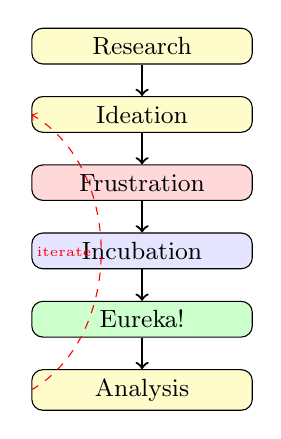
\begin{tikzpicture}[node distance=0.4cm, box/.style={draw, rounded corners, minimum width=2.8cm, minimum height=0.45cm, font=\small}]
\node[box, fill=yellow!20] (r) {Research};
\node[box, fill=yellow!20, below=of r] (i) {Ideation};
\node[box, fill=red!15, below=of i] (f) {Frustration};
\node[box, fill=blue!10, below=of f] (inc) {Incubation};
\node[box, fill=green!20, below=of inc] (e) {Eureka!};
\node[box, fill=yellow!20, below=of e] (a) {Analysis};

\foreach \a/\b in {r/i, i/f, f/inc, inc/e, e/a}
  \draw[->, thick] (\a) -- (\b);
\draw[->, dashed, red, bend right=60] (a.west) to node[left, font=\tiny, red]{iterate} (i.west);
\end{tikzpicture}
\end{center}

\vspace{4pt}
\textbf{Key elements for creative success} (George A.\ Wood Jr.):
\begin{enumerate}
  \item Solid basic knowledge (physics, math, chemistry).
  \item Ability to \textbf{visualize}.
  \item Building knowledge through experience and curiosity.
  \item Ability to \textbf{communicate} to technical and non-technical audiences.
  \item Knowledge of the physical result of engineering.
\end{enumerate}
\pref{21--25}
\end{frame}

% ============================================================
% 1.12 WHAT'S TO COME
% ============================================================

\begin{frame}
\frametitle{What's to Come: Course Roadmap}

\textbf{Part~I --- Kinematics of Mechanisms:}
\begin{itemize}
  \item \textbf{Synthesis} of mechanisms to accomplish desired motions or tasks.
  \item \textbf{Analysis} of mechanisms for kinematic behavior.
\end{itemize}

\vspace{6pt}
\textbf{Part~II --- Dynamics of Machinery:}
\begin{itemize}
  \item \textbf{Dynamic analysis} of forces and torques generated by moving machines.
\end{itemize}

\vspace{6pt}
\begin{yellowbox}
\textbf{Sequence:} Synthesis $\to$ kinematic analysis $\to$ dynamic analysis.

Once the kinematics and kinetics have been determined, most of the conceptual design is complete. What remains is \textbf{detailed design} --- sizing parts against failure.
\end{yellowbox}
\pref{25--26}
\end{frame}

\begin{frame}
\frametitle{Chapter Overview: The Big Picture}

\begin{center}
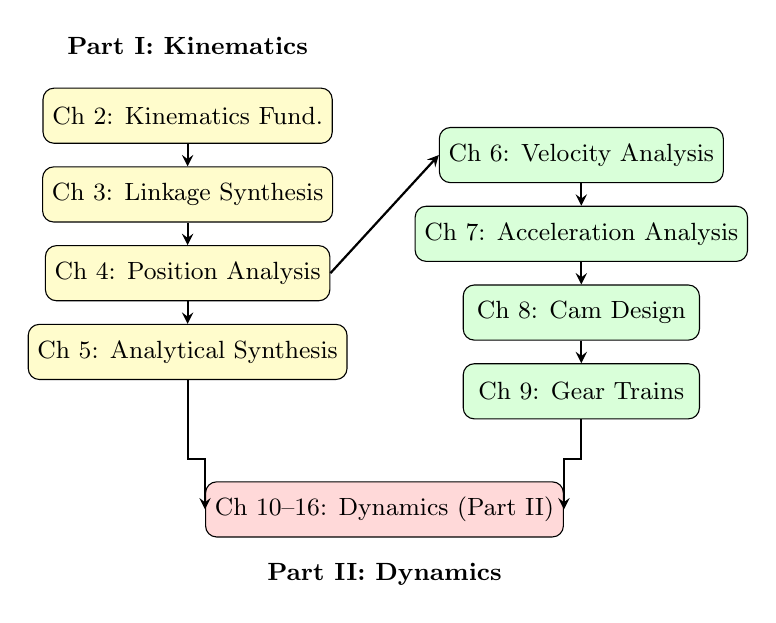
\begin{tikzpicture}[
  block/.style={draw, rounded corners, minimum width=3cm, minimum height=0.7cm, text centered, font=\small},
  arrow/.style={->, thick, >=stealth}
]
\node[block, fill=yellow!20] (ch2) at (0,0) {Ch 2: Kinematics Fund.};
\node[block, fill=yellow!20] (ch3) at (0,-1) {Ch 3: Linkage Synthesis};
\node[block, fill=yellow!20] (ch4) at (0,-2) {Ch 4: Position Analysis};
\node[block, fill=yellow!20] (ch5) at (0,-3) {Ch 5: Analytical Synthesis};
\node[block, fill=green!15] (ch6) at (5,-0.5) {Ch 6: Velocity Analysis};
\node[block, fill=green!15] (ch7) at (5,-1.5) {Ch 7: Acceleration Analysis};
\node[block, fill=green!15] (ch8) at (5,-2.5) {Ch 8: Cam Design};
\node[block, fill=green!15] (ch9) at (5,-3.5) {Ch 9: Gear Trains};

\node[block, fill=red!15] (ch10) at (2.5,-5) {Ch 10--16: Dynamics (Part II)};

\draw[arrow] (ch2) -- (ch3);
\draw[arrow] (ch3) -- (ch4);
\draw[arrow] (ch4) -- (ch5);
\draw[arrow] (ch4.east) -- (ch6.west);
\draw[arrow] (ch6) -- (ch7);
\draw[arrow] (ch7) -- (ch8);
\draw[arrow] (ch8) -- (ch9);
\draw[arrow] (ch9.south) -- ++(0,-0.5) -| (ch10.east);
\draw[arrow] (ch5.south) -- ++(0,-1) -| (ch10.west);

\node[above=0.3cm of ch2, font=\small\bfseries] {Part I: Kinematics};
\node[below=0.2cm of ch10, font=\small\bfseries] {Part II: Dynamics};
\end{tikzpicture}
\end{center}

\end{frame}

% ============================================================
% SUMMARY
% ============================================================

\begin{frame}
\frametitle{Chapter 1: Summary of Key Concepts}

\begin{enumerate}
  \item \textbf{Kinematics} $=$ study of motion (no forces); \textbf{Kinetics} $=$ study of forces in motion. Linked by $\mathbf{F} = m\,\mathbf{a}$.
  \item \textbf{Mechanism} $=$ transmits motion (low force); \textbf{Machine} $=$ transmits motion + significant force/power.
  \item The \textbf{design process} is a structured, 10-step, \textbf{iterative} approach to solving unstructured engineering problems.
  \item \textbf{Functional visualization} and the \textbf{creative process} (idea generation $\to$ frustration $\to$ incubation $\to$ Eureka!) are essential.
  \item The \textbf{decision matrix} is a tool for systematically comparing design alternatives.
  \item \textbf{Units} matter: fps (slugs), ips (blobs), SI (kg). Always check dimensional consistency.
  \item \textbf{Communication} is as important as computation.
\end{enumerate}

\end{frame}

\begin{frame}
\frametitle{Key Definitions to Remember}

\begin{yellowbox}
\begin{tabular}{@{}ll@{}}
\textbf{Kinematics} & Study of motion without regard to forces \\
\textbf{Kinetics} & Study of forces on systems in motion \\
\textbf{Mechanism} & System of elements to transmit motion \\
\textbf{Machine} & Mechanism with significant force/power \\
\textbf{Synthesis} & Putting together; creating \\
\textbf{Analysis} & Taking apart; evaluating \\
\textbf{Iteration} & Repeating; returning to a previous state \\
\textbf{Slug} & lb-sec$^2$/ft (fps mass unit) \\
\textbf{Blob} & lb-sec$^2$/in (ips mass unit); $= 12$ slugs \\
\textbf{Ergonomics} & Human factors engineering \\
\textbf{Functional viz.} & Visualize function, not embodiment \\
\end{tabular}
\end{yellowbox}

\end{frame}

\begin{frame}
\frametitle{Self-Check Questions}

Test your understanding of this chapter:

\begin{enumerate}
  \item What is the difference between a mechanism and a machine?
  \item Why do we study kinematics before kinetics?
  \item What are the 10 steps of the design process? Why is it iterative?
  \item What is ``functional visualization'' and why is it important?
  \item Describe the four phases of the creative process.
  \item What is a decision matrix and what is its primary value?
  \item What are the three unit systems discussed? What are their base units?
  \item Why is the blob--slug distinction critical? Give a numerical example.
  \item What role does communication play in engineering design?
  \item Describe the key insight in Towfigh's fourbar linkage design.
\end{enumerate}

\end{frame}

\end{document}
